\documentclass[aspectratio=169,dvipsnames]{beamer}

%\usepackage[czech]{babel}
\usepackage{polyglossia}
\setmainlanguage{czech}
\usepackage[nounicodemath,czech]{ufalslides}
\usepackage{xcolor}
\usepackage{textcomp}
\usepackage{booktabs}
\usepackage{collcell}
\usepackage{xstring}
\usepackage{tikz-dependency}
\usepackage{amssymb}

%\usepackage{csquotes}
%\usepackage[citestyle=authoryear]{biblatex}


%\makeatletter
%\def\blx@nowarnpolyglossia{1}
%\makeatother

\usepackage{tikz}
\usepackage{gnuplot-lua-tikz}
\usepackage{tikz-qtree}
\usetikzlibrary{calc}
\usetikzlibrary{arrows,shapes,positioning}
\usetikzlibrary{arrows.meta}

\setbeamercolor{blockcolor}{bg=gray!20, fg=black}


% %%%%%%%%%%%%%%%%%%%%%%%%%%%%%%%%%%%%%%%%%%%%%%%%%%%%%%%%%%%%%%%%%%%%%%%%%%%%%
\def\course{NAIL127 AI v Kontextu}
\def\courseurl{https://ufal.mff.cuni.cz/AIvK}
\def\title{Úvodní přednáška}
\def\subtitle{Co je a není AI, co je strojové učení a neuronové sítě}
\def\author{Tereza Hanemann, \underline{Jindřich Libovický}, Rudolf Rosa}
\def\date{19. února 2026}
\def\licence{cc-by-nc-sa}
\def\showtitleoneveryframe{}
%\def\langtech{}
\def\shownavigation{}
% %%%%%%%%%%%%%%%%%%%%%%%%%%%%%%%%%%%%%%%%%%%%%%%%%%%%%%%%%%%%%%%%%%%%%%%%%%%%%

\begin{document}

\maketitle

\section{AI v Kontextu}

\begin{frame}{Tým AI v kontextu}

    \begin{minipage}{70pt}
    \begin{tikzpicture}
    \clip (0,0) circle (30pt);
    \node at (0.0,-0.10) {\includegraphics[scale=0.3]{img/tereza.jpg}};
    \end{tikzpicture}
    \end{minipage}\begin{minipage}{200pt}
        \textbf{Tereza Hanemann} \\
        \textit{Katedra softwaru a výuky informatiky} \\
        \quad$\bullet$ vývoj počítačových her \\
        \quad$\bullet$ didaktika informatiky
    \end{minipage}

    \vspace{10pt}

    \hspace{40pt}\begin{minipage}{70pt}
    \begin{tikzpicture}
    \clip (0,0) circle (30pt);
    \node at (0.0,-0.75) {\includegraphics[scale=0.35]{img/rudolfrosa.png}};
    \end{tikzpicture}
    \end{minipage}\begin{minipage}{250pt}
        \textbf{Rudolf Rosa} \\
        \textit{Ústav formální a aplikované lingvistiky} \\
        \quad$\bullet$ analýza chování neuronových sítí \\
        \quad$\bullet$ generování literárních textů
    \end{minipage}

    \vspace{10pt}

    \hspace{80pt}\begin{minipage}{70pt}
    \begin{tikzpicture}
    \clip (0,0) circle (30pt);
    \node at (0.0,-0.35) {\includegraphics[scale=0.35]{img/jindrich.jpg}};
    \end{tikzpicture}
    \end{minipage}\begin{minipage}{250pt}
        \textbf{Jindřich Libovický} \\
        \textit{Ústav formální a aplikované lingvistiky} \\
        \quad$\bullet$ vícejazyčné jazykové modely \\
        \quad$\bullet$ férovost jazykových modelů napříč jazyky
    \end{minipage}

\end{frame}

% ----------------------------------------------------------------------------

%\begin{frame}{Organizace předmětu}

    \begin{itemize}[<+->]

        \item Úvodní přednáška -- \textbf{teď}

        \begin{itemize}[<+->]

            \item Technický úvod, co je a není AI

            \item Základy strojového učení a neuronových sítí

            \item Ukázky z~počítačového vidění a zpracování jazyka

        \end{itemize}

		\item Seminář o obecných otázkách 9.4.

        \item Přednášky: host mluví na dané téma
            \hfill 26.2. \quad 12.3. \quad 26.3. \quad 16.4. \quad 30.4.

        \item Semináře: téma předchozí přednášky, obvykle založené na čtení
            nějaké literatury \\
            \hfill \phantom{0}5.3. \quad 19.3. \quad \phantom{0}2.4. \quad 23.4. \quad \phantom{0}7.5.

        \item Na závěr (21.5.) shrnutí a závěrečný test

    \end{itemize}

    \vspace{5pt}

    \centering
    \visible<8->{\fbox{\begin{minipage}{.9\textwidth}
        \Large Zápočet: \\ ~$\bullet$ \textbf{účast} na 4 přednáškách a 4 seminářích \\ ~$\bullet$ \textbf{závěrečný test} (pouze informativní)
    \end{minipage}}}

\end{frame}
% ----------------------------------------------------------------------------

\begin{frame}{Program}

    \small\centering
    \begin{tabular}{cl}
        \toprule
    Datum   &   Program \\ \midrule
     19.2. & Úvodní přednáška \\ \midrule

    26.2. & ??: \hfill \textbf{AI a divadlo}  \\
     5.3. & Seminář (RR) \\ \midrule

	12.3. & Jana Soukupová (PrF UK): \hfill \textbf{Právní aspekty AI v kontextu vzdělávání} \\
    19.3. & Seminář (RR) \\ \midrule

	26.3. & Karl Štěpánová (CIIRC ČVUT): \hfill \textbf{Adaptivní robotické systémy: Učení a přizpůsobování napříč úlohami a uživateli} \\
	 2.4. & Seminář (TH) \\ \midrule

	9.4. & Seminář o obecných otázkách spojených s AI (JL) \\ \midrule

    16.4. & Josef Šlerka (FF UK) \hfill \textbf{AI v~kontextu sociologie}  \\
    23.4. & Seminář (TH) \\ \midrule

    30.4. & Marek Urban (PSÚ AV ČR) \hfill \textbf{AI ve vzdělávání} \\
     7.5. & Seminář (JL) \\ \midrule

    14.5. & Speciální seminář (TH) ¨

    21.5. & Závěrečné shrnutí a test \\
    \bottomrule
    \end{tabular}

\end{frame}


% ----------------------------------------------------------------------------

\begin{frame}{Domácí příprava}

    \begin{itemize}[<+->]

        \item Konkrétní \textbf{zadání během pátku} po přednášce

        \item Četba, otázky na rozmyšlení, drobnější aktivity

        \item Odpovědi/výsledky \textbf{posílat prostřednictím formuláře}

        \item Obvyklý deadline je \textbf{středa 12:00} následujícího týdne

    \end{itemize}

    \vspace{10pt}

    \centering
    \visible<5->{\fbox{\begin{minipage}{.9\textwidth}
        \centering\Large Na zápočet je potřeba odevzdat alespoň 4$\times$ za semestr.
     \end{minipage}}}

\end{frame}

% ----------------------------------------------------------------------------
\begin{frame}{Diskusní semináře}

\begin{itemize}

    \item Diskuse nebo aktivity v~malých skupinkách

    \item Předmět navševují lidé z~různách oborů a různých stupňů studia: nemůžeme předpokládat, sdílenou (technickou) znalost

    \item Nechte předsudky doma

\end{itemize}

\vspace{10pt}

\begin{center}
    \visible<2->{\fbox{\begin{minipage}{.9\textwidth}

        \centering\Large Diskutujte slušně a s~respektem k~různým názorům.

     \end{minipage}}}
\end{center}

\end{frame}


\section[Co je AI]{Co je umělá inteligence}

% ----------------------------------------------------------------------------

\begin{frame}{Ne-definice}

    \begin{center}
        \Large
    \textbf{Umělá inteligence} = obor informatiky, který se zabývá řešením
    úloh\ldots
    \end{center}

    \vspace{10pt}

    \begin{itemize}

        \item<2-> O kterých se vágně shodneme, že k~jejich řešení lidé potřebují
            inteligenci

        \item<3-> Někdy úlohy, které vyžadují \textbf{velké mentální úsilí} \\
            \quad \emph{hraní šachů nebo Go, automatický překlad}

        \item<4-> Někdy úlohy, které jsou \textbf{pro člověka triviální} \\
            \quad \emph{rozpoznávání objektů na fotografii, rozpozávání řeči}

    \end{itemize}

    \centering\vspace{15pt}

    \visible<5->{Hranice, co se považuje AI, se posouvá sem a tam\ldots}

\end{frame}

% ----------------------------------------------------------------------------

\begin{frame}{Exponenicálně rostoucí obor}

    \centering
    \includegraphics[scale=.25]{./img/exp_growth.jpg}

    Počet publikovaných článeků se každé dva roky zdvojnásobí.

    {\footnotesize Zdroj: \citet{krenn2022prediction}}

\end{frame}

% ----------------------------------------------------------------------------

\begin{frame}{Společensko-vědní pohled}

    \begin{quote}
        [T]he phrase “artificial intelligence” is deployed when the people building
        or selling a particular set of technologies will profit from getting others
        to believe that their technology is similar to humans, able to do things
        that, in fact, intrinsically require human judgment, perception, or
        creativity.
    \end{quote}

    {\footnotesize Zdroj: \citet{bender2025ai}}

\end{frame}

% ----------------------------------------------------------------------------

\begin{frame}{Inteligentní chování = AI?}

    \begin{columns}
        \column{.40\textwidth}
        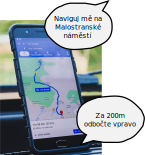
\includegraphics[scale=0.45]{./img/navigation.pdf}

        \column{.55\textwidth}

        \begin{enumerate}

            \item<2-> Rozpoznávání řeči \\
                \visible<9->{\hfill\it\color{gray} neuronová síť naučená z nahrávek}

            \item<3-> Analýza textu \\
                \visible<10->{\hfill\it\color{gray} pravidla nebo neuronová síť}

            \item<4-> Vyhledání cíle na mapě \\
                \visible<11->{\hfill\it\color{gray} vyhledávání v databázi, spíš SW inženýrství}

            \item<5-> Nalezení nejlepší cesty \\
                \visible<12->{\hfill\it\color{gray} optimalizace, diskrétní matematika}

            \item<6-> Určení polohy, rozhodnutí co je další krok na nejlepší cestě
                \visible<13->{\hfill\it\color{gray} jednoduchý algoritmus}

            \item<7-> Generování přirozeného jazyka \\
                \visible<14->{\hfill\it\color{gray} jednoduchý algoritmus nebo neuronová síť}

            \item<8-> Syntéza řeči \\
                \visible<15->{\hfill\it\color{gray} neuronová síť naučená z nahrávek}

        \end{enumerate}

    \end{columns}

\end{frame}

% ----------------------------------------------------------------------------

\begin{frame}{Strong vs. Weak AI}

    \begin{columns}[t]
        \column{.45\textwidth}
        \begin{center}
        \visible<1->{{\Large \textbf{Strong AI}}}
        \end{center}

        \vspace{5pt}

        \begin{itemize}

            \item<2-> Také AGI -- \\ \quad Artifitial General Inteligence

            \item<3-> Cílem je obecně \textbf{inteligentní stroj}, který v důsledku
			    toho umí řešit \textbf{všechny úlohy}

            \item<4-> (Ne)vědecký/(ne)inženýrský koncept

        \end{itemize}


        \column{.45\textwidth}
        \begin{center}
        \visible<5->{{\Large \textbf{Weak AI}}}
        \end{center}

        \vspace{5pt}

        \begin{itemize}

            \item<6-> Také Narrow AI

            \item<7-> Cílem je řešit \textbf{jednotlivé úlohy}, které vyžadují
					(lidskou) inteligenci

            \item<8-> Všechno, o čem bude dnes řeč, je weak AI

        \end{itemize}

		\vspace{15pt}

			\visible<9->{Co je inteligence a co je jenom počítání?}

    \end{columns}


\end{frame}

% ----------------------------------------------------------------------------

\begin{frame}{Superintelligence: Pojem inteligence je problematický}

    \begin{itemize}

        \item<1-> Moderní pojetí inteligence jako jedné měřitelné veličiny vzniklo
            z velké části v kontextu \textbf{eugenického hnutí} (konec 19. a začátek 20. století)

            \begin{itemize}
                \item<2-> Eugenici potřebovali lidi \emph{seřadit} -- nutně tedy
                    jednodimenzionální škála
                \item<3-> IQ testy často sloužily jako nástroj k odůvodnění
                    sociální nerovnosti
            \end{itemize}

        \item<4-> Skutečná lidská inteligence je \textbf{mnohodimenzionální}

            \begin{itemize}
                \item<5-> Gardnerova teorie mnohočetných inteligencí \\
                    \quad {\small\it jazyková, logická, prostorová, hudební, tělesná\ldots}
                \item<6-> Sternbergův triarchický model \\
                    \quad {\small\it analytická, kreativní, praktická}
            \end{itemize}

        \item<7-> Říct, že někdo nebo něco je „inteligentnější", \textbf{nedává
            jednoznačný smysl}

            \begin{itemize}
                \item<8-> Inteligentnější \emph{v čem} a \emph{pro jaký účel}?
                \item<9-> Šachový program poráží každého velmistra~-- je tedy
                    „inteligentnější než člověk"?
            \end{itemize}

    \end{itemize}

\end{frame}


% ----------------------------------------------------------------------------

%\begin{frame}{Strong AI: Turingův test}
%
%\end{frame}
%
%% ----------------------------------------------------------------------------
%
%\begin{frame}{Strong AI: Čínský pokoj}
%
%\end{frame}

% ----------------------------------------------------------------------------

\begin{frame}{Když se dneska řekne AI}

    \Large

    \begin{itemize}[<+->]

        \item Většinou jsou to metody založené na \textbf{strojovém učení}  \\  \quad a zpracování
            \textbf{hodně dat} \\[1em]

        \item Často je to strojové učení pomocí \textbf{neuronových sítí} \\[1em]

        \item Fantazie/marketing CEOs technologických firem a hype médií
            \visible<4->{\hfill\it\color{gray} (a někdy i vědců)} \\[1em]

    \end{itemize}


\end{frame}


\section[Strojové učení]{Strojové učení \& Neuronové sítě}

\begin{frame}{Běžné programování vs.\ strojové učení}

    {\large \textbf{Programování řešení}}

    \begin{itemize}

        \item<2-> Jsme schopni problém \textbf{formálně popsat} jasnými koncepty

        \item<3-> Program je jednoznačný \textbf{návod}, jak s koncepty zacházet

    \end{itemize}

    \vspace{10pt}

    \visible<4->{%
    \begin{beamercolorbox}{blockcolor}
    {\color{ufal} Příklad -- E-shop:} {\it Koncepty: zboží, sklad, zákazník,
    objednávka} \\
    \quad Udělat objednávku, odeslat objednávku = jednoduchý algoritmus
    \end{beamercolorbox}}

    \vspace{20pt}

    \visible<5->{{\large \textbf{Učení řešení}}}

    \begin{itemize}

	    \item<6-> Máme \textbf{příklady} vstupů a výstupů a \textbf{metriku} jak dobré je řešení

        \item<7-> Nejsme schopni do důsledku napsat návod, jak úlohu řešit

    \end{itemize}

    \vspace{10pt}

    \visible<8->{%
    \begin{beamercolorbox}[]{blockcolor}
    {\color{ufal} Příklad -- automatický překlad:} {\it neexistuje návod, pro člověka, který nerozumí oběma jazykům} \\
    \quad Existuje mnoho přeložených textů, co se dají použít pro trénování
    \end{beamercolorbox}}

\end{frame}

% ----------------------------------------------------------------------------

\begin{frame}{Obecné schéma}

    \centering
\scalebox{.8}{%
\begin{tikzpicture}%
[   normal arrow/.style={draw,-triangle 45,very thick},
    big box/.style={draw=####1!20!black, fill=####1!60, minimum width=9em, minimum height=9em, rectangle, align=center},
    small box/.style={draw, minimum height=5mm, minimum width=####1, rectangle}
]
\node[big box = RoyalBlue] (d) at (1, -5) {};
\node[above] at (d.north) {};
\node[below, align=center] at (d.north) {data};
\node[big box = ForestGreen] (a) at (7, -5) {};
\node[below, align=center] at (a.north) {učící algoritmus};
\node[big box = Dandelion] (m) at (14, -5) {};
\node[below, align=center] at (m.north) {model};

\path[normal arrow] (d) -- (a);
\path[normal arrow] (a) -- (m);

\foreach \x in {1,...,3} {%
	\node[small box = 5em] (x\x) at (0.4, -3.4 - \x * 0.8) {$x_{\x}$};
	\node[small box = 1.5em] (y\x) at (2.2, -3.4 - \x * 0.8) {$y_{\x}$};
	\path[draw] (x\x) -- (y\x);
}
\node[] (xc) at (0.4, -3.2 - 4 * 0.8) {$\vdots$};
\node[] (yc) at (2.2, -3.2 - 4 * 0.8) {$\vdots$};

\node[small box = 5em] (x) at (14, -2) {$x$};
\node[small box = 1.5em] (y) at (14, -8) {$y$};

\path[normal arrow] (x) -- (m);
\path[normal arrow] (m) -- (y);

\node[small box = 6em] (meta) at (7, -5) {hyperparametry};

\node[small box = 6em] (par-alg) at (14, -5) {parametery};
\node[small box = 6em] (par) at (14, -6) {algoritmus};

\end{tikzpicture}}

    \vspace{1em}

    \visible<2->{Cíl učení = model, který \textbf{generelalizuje} pro nová data.}

\end{frame}

% ----------------------------------------------------------------------------

\begin{frame}{Příklad strojového učení}

    \centering
    \begin{tabular}{lcc}
        & \visible<1->{\bf Rozpoznávání objektů & \bf Strojový překlad} \\ \midrule

        \visible<2->{
        \bf Data & $x$: RGB obrázek           & $x$: Věta ve zrdojovém jazyce \\
             & $y$: Pozice a typ objektu  & $y$: Věta v cílovém jazyce \\ \midrule}

         \visible<3->{
        \bf Učící algoritmus & \multicolumn{2}{c}{Minimalizace chyby, gradient descent} \\ \midrule}

    \visible<4->{
        \bf Model & konvoluční neuronová síť & Transformer (neuronová síť)  \\ \midrule}

    \visible<5->{
    \bf Algoritmus & sliding window přes obrázek & autoregresivní dekódování \\
               & (obdélníky různých velikostí) & (vždy jedno slov na výstup, \\
               &  & jde na vstup v dalším kroku)}

    \end{tabular}


\end{frame}

% ----------------------------------------------------------------------------

\begin{frame}{Generalizace vs. přeučení}

    \begin{center}
    \includegraphics{./img/overfitting.png} \\
    {\tiny Zdroj: https://www.geeksforgeeks.org/underfitting-and-overfitting-in-machine-learning}
    \end{center}

    \visible<2->{
        \textbf{\Large Přeučení} = model si zapamatuje trénovací data, funguje dobře jenom pro data, která vypadají jako trénovací} \\
    \visible<3->{\hfill \Large\bf \ldots nejčastější zdroj chyb a diskriminace}

\end{frame}

% ----------------------------------------------------------------------------

\begin{frame}{Neuronové sítě: Jeden neuron}

    \begin{columns}
        \column{.45\textwidth}
        \begin{tikzpicture}[]

\tikzset{>=latex}
\def\inputX{-4.0}
\def\labelY{-2.6}

\draw (0,\labelY - 0.2) node {aktivační};
\draw (0,\labelY + 0.2) node {funkce};

\draw (\inputX,\labelY) node {vstup $\mathbf{x}$};

\draw (\inputX / 2,\labelY) node {parametry $\mathbf{w}$};

\draw (2.0, \labelY) node {výstup};


\draw (0,0) node[draw,circle](neuron) {$\sum \mathbf{x}^\top\mathbf{w} > 0$?};
    \draw[->] (neuron) -- (2,0) node {~~~~~y};

\draw (\inputX,0) node {$x_i$} edge[->] node[anchor=north, pos=.5] {$\cdot w_i$} (neuron);

\draw (\inputX,2.0) node {$x_1$} edge[->]
    node[anchor=south, pos=.5] {$\cdot w_1$} (neuron);
\draw (\inputX,1.2) node {$x_2$} edge[->]
    node[anchor=south, pos=.5] {$\cdot w_2$} (neuron);

\draw (\inputX,0.8) node {$\vdots$};

\draw (\inputX,-0.9) node {$\vdots$};

\draw (\inputX,-1.8) node {$x_n$} edge[->]
    node[anchor=north, pos=.5, below] {$\cdot w_n$} (neuron);

\end{tikzpicture}

        \column{.45\textwidth}

        \begin{itemize}[<+->]

            \item Vstupy = reálná čísla

            \item Smíchají s různými vahami

            \item Začátek v 50.\ letech, inspirace představou o neuronu
                ze 40.\ let

            \item Dnes \textbf{nic společného} s biologickými neurony

        \end{itemize}

    \end{columns}

\end{frame}

% ----------------------------------------------------------------------------

\begin{frame}{Neuronová síť: Více vrstev}

    \centering
    Úloha: rozpoznat písmeno z~mřížky 4$\times$4 pixely

    \vspace{10pt}

    \includegraphics{./img/feedforward.pdf}

\end{frame}

% ----------------------------------------------------------------------------

\begin{frame}{Neuronová síť}

    \begin{columns}
        \column{.4\textwidth}

        \scalebox{.75}{\def\layerA{7}
\def\layerB{9}
\def\layerC{9}
\def\layerD{3}
\def\step{2}
\def\size{3pt}

\begin{tikzpicture}[]


\foreach \i in {0,...,\layerA} {
	\draw (0,-0.25 -0.4 * \i) circle (\size) node(layer_1_\i) {};
}
\draw (0, 0.5) node {\small vstup};

\foreach \i in {0,...,\layerB} {
	\draw (\step,-0.4 * \i) circle (\size) node(layer_2_\i) {};
}

\foreach \i in {0,...,\layerC} {
	\draw (2 * \step,-0.4 * \i) circle (\size) node(layer_3_\i) {};
}

\draw (1.5 * \step, 0.5) node {\small skryté vrstvy};

\foreach \i in {0,...,\layerD} {
	\draw (3 * \step,-1 - 0.4 * \i) circle (\size) node(layer_4_\i) {};
    \draw[->] (layer_4_\i) -- (3 * \step + 0.4, -1 - 0.4 * \i);
}

\draw (3 * \step, 0.5) node {\small výstup};

\foreach \i in {0,...,\layerA} {
	\foreach \j in {0,...,\layerB} {
        \draw[->] (layer_1_\i) -- (layer_2_\j);
    }
}

\foreach \i in {0,...,\layerB} {
	\foreach \j in {0,...,\layerC} {
        \draw[->] (layer_2_\i) -- (layer_3_\j);
    }
}

\foreach \i in {0,...,\layerC} {
	\foreach \j in {0,...,\layerD} {
        \draw[->] (layer_3_\i) -- (layer_4_\j);
    }
}

\end{tikzpicture}
}

        \column{.5\textwidth}
        \begin{itemize}[<+->]

            \item Organizace do vrstev $\Rightarrow$

            \begin{itemize}[<+->]

                \item Na vstup vrstvy $\sim$ vektor

                \item Vážení vstupů $\sim$ maticové násobení

                \item Výstup vrstvy $\sim$ vektor

            \end{itemize}

        \item Většina výpočtů \textbf{maticové násobení} $\Rightarrow$ rychlé počítání
            na GPU

        \item Výstup NN = \textbf{spojitá funkce} vstupů

        \end{itemize}
    \end{columns}

\end{frame}

% ----------------------------------------------------------------------------

\begin{frame}{Chybová funkce \& Trénování}

    \begin{itemize}[<+->]

        \item Trénování = \textbf{minimalizace chyby} na trénovacích datech

        \item Když je chyba \textbf{spojitá funkce}, můžeme spočítat
            \textbf{derivaci chyby} vzhledem k parametrům

        \item Posunout parametry po směru derivace = snížit chybu

    \end{itemize}

\end{frame}

% ----------------------------------------------------------------------------

\begin{frame}{Problematická trénovací data}

    \visible<1->{
    {\Large\textbf{Stahování z internetu}} --- neprezentativní, extrémní názory
    jsou mnohem víc slyšet, není kontrola nad tím, co je v datech
    \\ \hfill {\footnotesize \citep{bender2021dangers}}}

    \vspace{15pt}

    \visible<2->{
    {\Large\textbf{Crowd-sourcing}} --- využívání levné pracovní síly, tzv. gig
    economy -- vznikají prekarizovaná zaměstnání
    \\ \hfill {\footnotesize \citep[kap. 2]{crawford2021atlas}}}

    \vspace{15pt}

    \visible<3->{
    {\Large\textbf{Vytěžování existujících databází}} --- neplacená práce
    uživatelů, neprůhledné využití dat (např. když za služby vyhledavače platíme daty)
    \\ \hfill {\footnotesize \citep{couldry2019costs}}}

\end{frame}

% ----------------------------------------------------------------------------

\begin{frame}{Problémy učení z dat: Overfitting}

    \begin{itemize}

        \item<1-> Optimalizované metriky nepostihnou všechno \\[1ex]
            \visible<2->{
            \quad\begin{minipage}{360pt}
                \it Vyhledávání vhodných kandidátů podle CV: když doporučím
                samé vhodné kandidáty, ani si nevšimnu, že jsem nedoporučil
                jiné vhodné (třeba podle rasy)
            \end{minipage} \\
            \hfill {\tiny \citep{derous2019your,bender2018data}}}

        \item<3-> Stereotypy můžou být pro model efektivní způsob optimalizace \\

            \visible<4->{
                \includegraphics[width=350pt]{img/doctor.png}} \\
            \visible<5->{
                \includegraphics[width=350pt]{img/sexy_doctor.png} \\
            \hfill {\tiny Příklad \citet[obr.\ 6 a 7]{rozhledy}} }

    \end{itemize}

\end{frame}

%\section{Počítačové vidění}

\begin{frame}{Úlohy počítačového vidění}

    \vspace{-5pt}
    \begin{center}
        \large Cokoli, co se dá zjistit z obrazu, např. \ldots
    \end{center}

    \visible<2->{
    \begin{columns}[t]
        \column{.3\textwidth}
        \centering \textbf{Rozpoznávání objektů} \\[1ex]
        \includegraphics[width=.98\textwidth]{img/object_detection.png} \\
        {\tiny Zdroj: \url{https://pjreddie.com/darknet/yolo}}

        \column{.3\textwidth}
        \centering \textbf{Odhad hloubky v obrazu} \\[1ex]
        \includegraphics[width=.98\textwidth]{img/monocular_depth.png} \\
        {\tiny Zdroj: \citet[s.\ 9250, obr.\ 1]{pillai2019super}}

        \column{.3\textwidth}
        \centering \textbf{Poloha lidského těla} \\[1ex]
        \includegraphics[width=.98\textwidth]{img/pose_detection.png} \\

        \begin{minipage}{\textwidth}
        \tiny Zdroj: \href{https://towardsdatascience.com/realtime-multiple-person-2d-pose-estimation-using-tensorflow2-x-93e4c156d45f}{\tt https://towardsdatascience.com/\\ realtime-multiple-person-2d-pose- \\ estimation-using-tensorflow2- \\ x-93e4c156d45f}
        \end{minipage}

    \end{columns}}

    \visible<3->{\begin{center}
        \large \ldots pro člověka většinou triviální úlohy
    \end{center}}

\end{frame}

% ----------------------------------------------------------------------------

\begin{frame}{Úlohy počítačového vidění}

    \visible<1->{\begin{center}
        \large \ldots ale i vyžadující expertní znalost.
    \end{center}}

    \visible<2->{
    \begin{columns}[t]
        \column{.45\textwidth}
        \centering \textbf{Detekce tuberkulózy} \\[1ex]
        \includegraphics[scale=.13]{img/tuberculosis.png} \\
        {\tiny Zdroj: \citet[obr.\ 3]{Pasa-et-al-2019}}

        \column{.45\textwidth}
        \centering \textbf{Katalogizace galaxií} \\[1ex]
    \includegraphics[scale=.15]{img/galaxies.png} \\
        {\tiny Zdroj: \citep[obr.\ 4]{gonzales2018galaxy}}
    \end{columns}}

    \centering
    \visible<3->{Pro počítač žádný rozdíl.}

\end{frame}

% ----------------------------------------------------------------------------

\begin{frame}{Konvoluční sítě}

    \begin{minipage}{.45\textwidth}
        \begin{itemize}[<+->]

            \item Základní nástroj pro zpracování obrazu neuronovými sítěmi

            \item Okénko, které jede přes obrázek a detekuje nějaké vzorce

            \item Mnoho vrstvev $\rightarrow$ vzorce vzorců vzorců\ldots

            \item Model si vytváří potřebné abstrakce

        \end{itemize}
    \end{minipage}\begin{minipage}{.45\textwidth}
        \centering
        \scalebox{0.7}{\input{img/convolution2d.pdf_tex}}
    \end{minipage}

\end{frame}

% ----------------------------------------------------------------------------

\begin{frame}{Hluboké konvoluční sítě}

    \begin{center}
        \scalebox{0.4}{\input{./img/alexnet.pdf_tex}}
    \end{center}

    \begin{itemize}[<+->]

        \item Hluboká architektura: konvoluce, max-pooling, residual connections,
            batch normalization, 50--150 vrstev

        \item Typicky ,,předtrénováno'' na velkých datech, pro jednotlivé úlohy
            se ,,dotrénovávají'' poslední vrstvy

    \end{itemize}

\end{frame}

% ----------------------------------------------------------------------------

\begin{frame}{ImageNet: rozpoznávání objektů}

    \begin{center}
        Dataset, který pomohl odstartovat revoluci ve strojovém učení.
    \end{center}

    \centering

    \includegraphics[scale=.34]{./img/imagenet.png} \\
    {\tiny Zdroj: \citet[obr.\ 1]{deng2009imagenet}}

    \visible<2->{14M obrázků, 1000 různých tříd}

\end{frame}

% ----------------------------------------------------------------------------

\begin{frame}{ImageNet challenge}

    \centering
    \begin{tikzpicture}[gnuplot]
%% generated with GNUPLOT 5.2p8 (Lua 5.3; terminal rev. Nov 2018, script rev. 108)
%% Po 31. ledna 2022, 18:45:58
\path (0.000,0.000) rectangle (13.000,7.000);
\gpcolor{color=gp lt color border}
\gpsetlinetype{gp lt border}
\gpsetdashtype{gp dt solid}
\gpsetlinewidth{1.00}
\draw[gp path] (1.504,0.616)--(1.531,0.616);
\draw[gp path] (12.447,0.616)--(12.420,0.616);
\node[gp node right] at (1.320,0.616) {0.00};
\draw[gp path] (1.504,1.629)--(1.531,1.629);
\draw[gp path] (12.447,1.629)--(12.420,1.629);
\node[gp node right] at (1.320,1.629) {0.05};
\draw[gp path] (1.504,2.641)--(1.531,2.641);
\draw[gp path] (12.447,2.641)--(12.420,2.641);
\node[gp node right] at (1.320,2.641) {0.10};
\draw[gp path] (1.504,3.654)--(1.531,3.654);
\draw[gp path] (12.447,3.654)--(12.420,3.654);
\node[gp node right] at (1.320,3.654) {0.15};
\draw[gp path] (1.504,4.666)--(1.531,4.666);
\draw[gp path] (12.447,4.666)--(12.420,4.666);
\node[gp node right] at (1.320,4.666) {0.20};
\draw[gp path] (1.504,5.679)--(1.531,5.679);
\draw[gp path] (12.447,5.679)--(12.420,5.679);
\node[gp node right] at (1.320,5.679) {0.25};
\draw[gp path] (1.504,6.691)--(1.531,6.691);
\draw[gp path] (12.447,6.691)--(12.420,6.691);
\node[gp node right] at (1.320,6.691) {0.30};
\node[gp node center] at (2.572,0.308) {$2011$};
\node[gp node center] at (3.906,0.308) {$2012$};
\node[gp node center] at (5.241,0.308) {$2013$};
\node[gp node center] at (6.575,0.308) {$2014$};
\node[gp node center] at (7.910,0.308) {$2015$};
\node[gp node center] at (9.244,0.308) {$2016$};
\node[gp node center] at (10.579,0.308) {$2017$};
\draw[gp path] (1.504,6.691)--(1.504,0.616)--(12.447,0.616)--(12.447,6.691)--cycle;
\node[gp node center,rotate=-270] at (0.016,3.653) {5-best error rate};
\gpfill{rgb color={0.114,0.188,0.459}} (2.071,0.616)--(3.073,0.616)--(3.073,5.821)--(2.071,5.821)--cycle;
\gpcolor{rgb color={0.114,0.188,0.459}}
\draw[gp path] (2.071,0.616)--(2.071,5.820)--(3.072,5.820)--(3.072,0.616)--cycle;
\gpfill{rgb color={0.114,0.188,0.459}} (3.406,0.616)--(4.408,0.616)--(4.408,3.718)--(3.406,3.718)--cycle;
\draw[gp path] (3.406,0.616)--(3.406,3.717)--(4.407,3.717)--(4.407,0.616)--cycle;
\gpfill{rgb color={0.114,0.188,0.459}} (4.740,0.616)--(5.742,0.616)--(5.742,2.953)--(4.740,2.953)--cycle;
\draw[gp path] (4.740,0.616)--(4.740,2.952)--(5.741,2.952)--(5.741,0.616)--cycle;
\gpfill{rgb color={0.114,0.188,0.459}} (6.075,0.616)--(7.077,0.616)--(7.077,2.117)--(6.075,2.117)--cycle;
\draw[gp path] (6.075,0.616)--(6.075,2.116)--(7.076,2.116)--(7.076,0.616)--cycle;
\gpfill{rgb color={0.114,0.188,0.459}} (7.409,0.616)--(8.411,0.616)--(8.411,1.339)--(7.409,1.339)--cycle;
\draw[gp path] (7.409,0.616)--(7.409,1.338)--(8.410,1.338)--(8.410,0.616)--cycle;
\gpfill{rgb color={0.114,0.188,0.459}} (8.744,0.616)--(9.746,0.616)--(9.746,1.223)--(8.744,1.223)--cycle;
\draw[gp path] (8.744,0.616)--(8.744,1.222)--(9.745,1.222)--(9.745,0.616)--cycle;
\gpfill{rgb color={0.114,0.188,0.459}} (10.078,0.616)--(11.080,0.616)--(11.080,1.073)--(10.078,1.073)--cycle;
\draw[gp path] (10.078,0.616)--(10.078,1.072)--(11.079,1.072)--(11.079,0.616)--cycle;
\gpcolor{color=gp lt color border}
\node[gp node left] at (1.836,6.128) {\footnotesize~err=.257};
\node[gp node left] at (3.170,4.025) {\footnotesize~err=.153};
\node[gp node left] at (4.505,3.260) {\footnotesize~err=.115};
\node[gp node left] at (5.839,2.424) {\footnotesize~err=.074};
\node[gp node left] at (7.174,1.646) {\footnotesize~err=.035};
\node[gp node left] at (8.508,1.530) {\footnotesize~err=.029};
\node[gp node left] at (9.843,1.380) {\footnotesize~err=.022};
\node[gp node left] at (1.836,6.497) {\footnotesize~\citet{sanchez_high-dimensional_2011}};
\node[gp node left] at (3.170,4.394) {\footnotesize~\citet{krizhevsky_imagenet_2012}};
\node[gp node left] at (4.505,3.629) {\footnotesize};
\node[gp node left] at (5.839,2.793) {\footnotesize~\citet{simonyan_very_2014}};
\node[gp node left] at (7.174,2.015) {\footnotesize~\citet{he_deep_2016}};
\node[gp node left] at (8.508,1.899) {\footnotesize};
\node[gp node left] at (9.843,1.749) {\footnotesize~\citet{hu_squeeze-and-excitation_2017}};
\node[gp node left] at (3.170,4.764) {\footnotesize\it~AlexNet};
\node[gp node left] at (5.839,3.163) {\footnotesize\it~VGG19};
\node[gp node left] at (7.174,2.385) {\footnotesize\it~ResNet};
\node[gp node left] at (9.843,2.119) {\scriptsize\it~Squeeze~and~Excitation};
\draw[gp path] (1.504,6.691)--(1.504,0.616)--(12.447,0.616)--(12.447,6.691)--cycle;
%% coordinates of the plot area
\gpdefrectangularnode{gp plot 1}{\pgfpoint{1.504cm}{0.616cm}}{\pgfpoint{12.447cm}{6.691cm}}
\end{tikzpicture}
%% gnuplot variables


\end{frame}

% ----------------------------------------------------------------------------

\begin{frame}{Předtrénované reprezentace}

    \begin{columns}

        \column{.45\textwidth}
        \centering

        Nejpodobnější vektory k reprezentaci z poslední vrstvy AlexNetu.

        \includegraphics[scale=0.25]{./img/alexnet_neighbors.png} \\
        {\tiny Zdroj: \citet[obr.\ 4]{krizhevsky_imagenet_2012}}

        % TODO: vyznačit sloupec a neighbors
        % TODO: zopakovat obrázek AlexNetu 


        \column{.45\textwidth}
    \begin{itemize}[<+->]

        \item Klasifikace obrázků se učí obecné rysy

        \item Prakticky všechny úlohy začínají s předtrénovaným modelem

        \item Postupně se nahrazuje unsupervised metodami

    \end{itemize}


    \end{columns}

\end{frame}

% ----------------------------------------------------------------------------

\begin{frame}{Problémy ImageNetu}

    \begin{itemize}[<+->]

        \item Založeno na lexikální databázi z 90.\ let -- reflektuje o čem se
            mluvilo v USA před 40 lety

        \item Není kulturně neutrální: anglické slovo \emph{shovel} v~severní
            Americe a v~jižní Africe \\ {\tiny obrázek z prezentace
            \citet{liu-etal-2021-visually}} \\
            \includegraphics[scale=.35]{img/shovel.png}

        \item Obsahuje obrázky ke nutně stereotypním konceptům jako {\tiny \citep[str.\ 109]{crawford2021atlas}} \\
            \quad\it ,,alcoholic,'' ,,ape-man,'' ,,crazy,'' ,,hooker''
    \end{itemize}

\end{frame}

% ----------------------------------------------------------------------------

%\begin{frame}{Rozpoznávání obličejů}
%\end{frame}


% ----------------------------------------------------------------------------

% ----------------------------------------------------------------------------
\section[Zpracování jazyka]{Zpracování přirozeného jazyka}
% ----------------------------------------------------------------------------

\begin{frame}{Co je zpracování přirozeného jazyka}

    \begin{center}

        \Large Úlohy, pro jejichž řešení je potřeba (do nějaké míry) \\ \textbf{rozumět
        lidskému jazyku}

    \end{center}

    \begin{itemize}[<+->]

        \item<2-> základní řešení lze obvykle jednoduše naprogramovat

        \item<3-> pro zvýšení úspěšnosti jsou potřeba stále složitější pravidla

        \item<4-> od určité úrovně si neporadíme bez strojového učení

    \end{itemize}

\end{frame}

% ----------------------------------------------------------------------------

\begin{frame}{Vyhledávání odpovědí na otázky}

    \centering
    \includegraphics[scale=.26]{img/qa.png} \\
    {\tiny Screenhot z~dema Allen Institute for AI \url{https://demo.allennlp.org/reading-comprehension/transformer-qa}}

\end{frame}

% ----------------------------------------------------------------------------

\begin{frame}{Kontrola pravopisu}

    \centering
    \includegraphics[scale=.3]{img/grammarly.png} \\
    {\tiny Zdroj: Webová reklama grammarly.com}

\end{frame}

% ----------------------------------------------------------------------------

\begin{frame}{Strojový překlad}

    \centering
    \includegraphics[scale=.4]{img/lindat.png} \\
    {\tiny Zdroj: Překladač CUBBIT \url{https://lindat.mff.cuni.cz/services/translation} \citep{popel2020transforming}}

\end{frame}

% ----------------------------------------------------------------------------

\begin{frame}{Entity extraction}

    \includegraphics[scale=.4]{./img/mona_lisa.png} \\
    {\tiny Zdroj: \url{https://dandelion.eu/semantic-text/entity-extraction-demo}}

    \vspace{10pt}

    \visible<2->{Podúlohy:}
    \begin{enumerate}

        \item<3-> Named entity recognition: nalézt v~textu řetězce, co obsahují
            pojmenované entity

        \item<4-> Entity linking: co entity znamenají (první pád, odkaz do
            databáze/na Wikipedii)

    \end{enumerate}

\end{frame}

% ----------------------------------------------------------------------------

\begin{frame}{Koncept embeddingu}

    \begin{columns}

    \column{.45\textwidth}
    \begin{itemize}[<+->]

        \item neuronové sítě potřebují spojité vstupy

        \item one-hot vektor: očíslujeme slova, 0/1 indikuje slovo \\[1em]
            \scalebox{.9}{\input{img/onehot.tex}}

        \item první vrstva = násobení maticí

    \end{itemize}
    \column{.45\textwidth}

        \visible<4->{
        \centering
        \scalebox{4}{\rotatebox{-90}{\Huge $\Rsh$}}

        \vspace{5pt}

        {\Large
        Každé \textbf{slovo} (nebo jiná jednotka) je reprezentovaná mnohodimenzionálním
        \textbf{vektorem}}}

        \vspace{15pt}

        \begin{itemize}

            \item<5-> učí se ,,mimochodem`` z dat

            \item<6-> mají zajímavé vlastnosti

        \end{itemize}

    \end{columns}

\end{frame}

% ----------------------------------------------------------------------------

\begin{frame}{Ukázka z překladače}
    \hspace*{-10pt}\includegraphics{./plots/tsne.pdf} \\
    \tiny Zdroj: \citet{rozhledy}
\end{frame}

% ----------------------------------------------------------------------------

\begin{frame}{Princip transformeru}

    \begin{columns}
    \column{.45\textwidth}

        \scalebox{.8}{\begin{tikzpicture}

    \foreach \i in {1,...,8}{
			\node[draw,inner sep=7pt,fill=Magenta!80] (A\i) at (\i, 0) {\i};
			\node[draw,inner sep=7pt,fill=ForestGreen!80] (B\i) at (\i, 2.25) {\i};
			\node[draw,inner sep=7pt,fill=Cerulean!80] (C\i) at (\i, 4.5) {\i};
	}

    \foreach \i in {1,...,8}{
		\foreach \j in {1,...,8}{
		    \pgfmathsetmacro{\lnW}{0.1 + random(0,10)/10};
			\draw[->, line width=\lnW, color=Gray, -{latex[width=2mm,length=3mm]}] (A\i.north) -- (B\j.south);
		    \pgfmathsetmacro{\lnW}{0.1 + random(0,10)/10};
			\draw[->, line width=\lnW, color=Gray, -{latex[width=2mm,length=3mm]}] (B\i.north) -- (C\j.south);
		}
	}

\end{tikzpicture}
}

    \column{.45\textwidth}
        \begin{itemize}[<+->]

            \item Mezi klasickými vrstvami tzv. \textbf{self-attention}

            \item Každé slovo se ,,podívá'' na ostatní slova a vezme si z~něj
                relevantní informace

            \item Na začátku: vektor reprezentuje \textbf{izolované} slovo \\
                Na konci: vektor reprezentuje slovo \textbf{v~kontextu} věty

        \end{itemize}

    \end{columns}

    \vspace{10pt}
    \visible<4->{\begin{center}Transformer původně představili \citet{vaswani2017attention} původně pro strojový překlad.\end{center}}

\end{frame}

% ----------------------------------------------------------------------------

%\begin{frame}{Encoder-decoder: Strojový překlad}
%
%    \begin{center}
%    \includegraphics[scale=0.55]{img/encoder_decoder.pdf}
%    \end{center}
%
%    \vspace{10pt}
%
%    \centering
%    \visible<2->{
%        Dekodér sbírá informace \textbf{z~předchozích slov} a \textbf{z~enkodéru}} \\
%    \tiny Koncept enkodéru-dekodéru: \citep{kalchbrenner2013recurrent,sutskever2014sequence,bahdanaou2015neural}
%
%%\end{frame}
%
% ----------------------------------------------------------------------------
%\begin{frame}{Zkreslení z dat}
%\end{frame}

% ----------------------------------------------------------------------------

\begin{frame}{Předtrénované modely v NLP}

    \centering
    \begin{tikzpicture}

            \visible<3->{\draw[dashed,Gray] (0, -100pt) -- (0, 100pt);}

            \node[draw,fill=Orange!80,inner sep=15pt] (bert) {\begin{tabular}{c}Language \\ model\end{tabular}};

            \visible<2->{
            \node (pre) [left=50pt of bert.west] {\large\bf 1. Pre-training};
            \node (pre2) [below=0pt of pre.south] {\small (jednou, na velkých datech, trvá dlouho)};
            \node[draw,ellipse,inner sep=1pt,fill=Gray!20] (unlabeled) [above left=30pt and 30pt of bert.north west] {\begin{tabular}{c}prostý \\ text\end{tabular}};
            \draw[->] (unlabeled.east) to[out=0,in=90] (bert.north);
            \node[draw,ellipse,inner sep=3pt,fill=Gray!20] (mlm) [below left=30pt and 30pt of bert.south west] {\begin{tabular}{c}masked LM  \\ \hline causal LM\end{tabular}};
            \draw[->] (bert.south) to[out=270,in=0] (mlm.east);}

            \visible<3->{
            \node (fine) [right=50pt of bert.east] {\large\bf 2. Finetuning};
            \node (fine2) [below=0pt of fine.south] {\small (malá data, rychle)};
            \node[draw,ellipse,inner sep=1pt,fill=Dandelion] (labeled) [above right=30pt and 30pt of bert.north east] {\begin{tabular}{c}data pro \\ specifickou \\ úlohu\end{tabular}};
            \draw[->] (labeled.west) to[out=180,in=90] (bert.north);
            \node[draw,ellipse,inner sep=3pt,fill=Dandelion] (loss) [below right=30pt and 30pt of bert.south east] {\begin{tabular}{c}task-specific \\ objective\end{tabular}};
                    \draw[->] (bert.south) to[out=270,in=180] (loss.west);}


    \end{tikzpicture}
\end{frame}

%\begin{frame}{Předtrénování: Masked Language Model}
%
%    \centering
%    \fbox{\large
%    \colorbox{lightgray}{All}
%    \colorbox{lightgray}{human}
%    \colorbox{lightgray}{being}
%    \colorbox{lightgray}{are}
%    \colorbox{lightgray}{born}
%    \only<1>{\colorbox{lightgray}{free}}%
%    \only<2>{\colorbox{GreenYellow}{free}}%
%    \only<3>{\colorbox{Rhodamine!30}{\texttt{MASK}}}%
%    \only<4>{\colorbox{Dandelion}{hairy}}%
%    \only<5->{\colorbox{GreenYellow}{free}}
%    \colorbox{lightgray}{and}
%    \colorbox{lightgray}{equal}
%    \colorbox{lightgray}{in}
%    \colorbox{lightgray}{dignity}
%    \colorbox{lightgray}{and}
%    \colorbox{lightgray}{rights}}
%
%    \vspace{20pt}
%
%    \begin{enumerate}
%
%        \item<2-> Náhodně vybereme slovo $\rightarrow$
%            \colorbox{GreenYellow}{free}
%
%        \item<3-> S~pravděpodobností 80\% ho nahradíme značku
%            \colorbox{Rhodamine!30}{\texttt{MASK}}
%
%        \item<4-> S~pravděpodobností 10\% ho nahradíme náhodným slovem $\rightarrow$
%            \colorbox{Dandelion}{hairy}
%
%        \item<5-> S~pravděpodobností 10\% ho necháme, jak je $\rightarrow$
%            \colorbox{GreenYellow}{free}
%
%    \end{enumerate}
%
%		\vspace{10pt}
%
%    \visible<6->{
%    Model se snaží uhádnout chybějící slovo \colorbox{GreenYellow}{free}}
%    \visible<7->{
%    \ldots aby to dokázal musí nějak ,,rozumět'' zbytku věty.}
%
%    \vspace{20pt}
%    \tiny Myšlenka Masked Language model, viz. \citet{devlin2019bert}
%
%\end{frame}

% ----------------------------------------------------------------------------

\begin{frame}{Pre-training -- Finetuning}

    \centering

    {\huge
		Většina state-of-the-art řešení v NLP používá \textbf{předtrénovaný} model
		občas dotrénovaný na datech specifických pro úlohu.}

    \vspace{30pt}

	Trend vývoje: lepší předtrénované modely, nižší potřeba specifických dat,
		instruction tuning

\end{frame}

% ----------------------------------------------------------------------------
\section{Velké jazykové modely}
% ----------------------------------------------------------------------------

\begin{frame}{Generativní jazykové modely}

    \begin{itemize}[<+->]

        \item GPT = Generative Pre-trained Transformer

        \item Model, který předpovídá, jaké slovo v textu může následovat \\
            \it v~projektu TheAItre ho použili ke generování divadelní hry

        \item GPT-3 je natrénovaný na 45TB textu (37 milionů Zločinů a trestů),
            má 175 miliard parametrů (1600$\times$ více než BERT)

            \begin{itemize}[<+->]

                \item 37M Zločinů a trestů by na ploše fotbalového hřiště
                    dosáhlo výšky 4.5m

                \item BERT by mohl běžet na GPU z~PlayStation 5

                \item GPT-3 by potřebovalo přes 100 PlayStationů

            \end{itemize}

	%\item Ještě větší modely: Gopher 280B param., 1.9TB textu,  {\small (DeepMind; \citealp{deepmind2021gopher})} , \\ \quad  PaLM 540B param.,  {\small (Google;  \citealp{google2022palm})}

		\item Neplatí, že čím větší model, tím lepší -- scaling laws ukazují,
				že menší model, co se déle trénuje, může být lepší

		\item Dnešní 8B modely fungují lépe než GPT-3

    \end{itemize}

\end{frame}

% ----------------------------------------------------------------------------

\begin{frame}{In-Context Learning}

    \begin{center}
        \visible<2->{{\color{gray} Šedý text je \textbf{vstup do modelu},} černý text je jak \textbf{model navázal}.} \\
        \fbox{\includegraphics[scale=.65]{img/fewshot.pdf}} \\
        \tiny Zdroj: \citet[obr.\ 3.17]{brown2020gpt}
    \end{center}

    \begin{itemize}

        \item<3-> Neprobíhá učení -- žádný update parametrů

        \item<4-> Jazykový model vidí příklad a pokračuje ve stejném stylu

    \end{itemize}

\end{frame}

% -----------------------------------------------------------------------------

\begin{frame}{Scaling Laws}

    \begin{center}
    Experimenty Chinchila Google DeepMindu: delší trénování může kompenzovat počet parametrů
    \citep[Figure~1]{hoffmann2022training}

    \vspace{5pt}
    \includegraphics[scale=.6]{img/chinchilla.pdf}

    \vspace{10pt}

    Používá LLaMA a LLaMA 2 od Meta: Srovnatelné jako GPT-3, ale má jenom 30B parametrů \\
    \citep{touvron2023llama}

    \end{center}

\end{frame}

% -----------------------------------------------------------------------------

\begin{frame}{Emergentní vlastnosti LM (1)}

    \centering
    \includegraphics[scale=.65]{img/emergent.pdf}\hspace{10pt}
    \rotatebox{90}{\begin{minipage}{200pt}
			Zdroj: \citet[obrázek 2]{wei2022emergent}
    \end{minipage}}

\end{frame}

% -----------------------------------------------------------------------------

\begin{frame}{Emergentní vlastnosti LM (2)}

    \begin{itemize}[<+->]

		\item Nové schopnosti jazykových modelů se \textbf{objevují s
				velikostí} -- musí se \textbf{objevit}

		\item Skeptický protiargument: Retrospektivně se dá najít
				\textbf{spojitá metrika}, která ukazuje, že změna je průběžná
					\citep{schaeffer2023emergent}

    \end{itemize}

\end{frame}

% ----------------------------------------------------------------------------

\begin{frame}{Férovost dat}

    \begin{center}

        \visible<1->{Modely potřebují \textbf{enormní množství textu}, které
        je jenom na Internetu\ldots}

        \visible<2->{\ldots Internet je plný \textbf{toxického obsahu}.}
    \end{center}

    \centering

    \visible<3->{
        GPT-2 navrhuje pokračování textu: \\
        \includegraphics[scale=.42]{./img/hitler.png}}

    {\tiny Vytvořeno pomocí \url{https://transformer.huggingface.co/doc/gpt2-large}, model: \citet{radford2019language}}


\end{frame}

% ----------------------------------------------------------------------------

\begin{frame}{Asistenti založení na LLM}

    \begin{columns}

    \column{.3\textwidth}
        \includegraphics[width=\textwidth]{img/ChatGPT.png}

    \column{.66\textwidth}
    \begin{itemize}[<+->]

        \item Chatbot -- program, který komunikuje s~člověkem v~přirozeném jazyce

        \item Společnost OpenAI spustila ChatGPT v~prosinci 2022, GPT-4 březen 2023

		\item Uzavřené komerční modely (Gemini, Claude AI) a trochu ovevřenější modely (LLaMA3, Mistral)

        \item Založený na jazykovém modelu dotrénovaný pro ,,řešení úloh`` podle instrukcí

    \end{itemize}

    \end{columns}

\end{frame}

% ----------------------------------------------------------------------------

\begin{frame}{InstructGPT: Předchůdce ChatGPT}
    \centering
    \includegraphics[width=.8\textwidth]{img/instructgpt.pdf} \\
    \tiny Zdroj \citet[Figure 2]{ouyang2022instruct}
\end{frame}

% ----------------------------------------------------------------------------

\begin{frame}{Zpětnovazebné učení}

    \centering
    \begin{tikzpicture}

        \node (prompt) {Prompt from dataset/logs};

        \node[inner sep=5pt,fill=ufallightblue, below=40pt of prompt,minimum height=50pt] (lm) {\begin{minipage}{100pt}\centering\large Language \\ model \end{minipage}};

        \draw[->] (prompt) -- (lm);

        \node[below=40pt of lm] (answer) {Sampled answer};

        \draw[->] (lm) -- (answer);

        \visible<2->{
        \node[inner sep=5pt,fill=ufalgreen, right=130pt of lm,minimum height=30pt] (reward) {\begin{minipage}{80pt}\centering Reward \\ model \end{minipage}};
        \draw[->] (answer.east) to[out=0,in=270, looseness=0.7] (reward.south);
        \draw[->] (prompt.east) to[out=0,in=90, looseness=0.7] (reward.north);
        }

        \visible<3->{
        \node[right=40pt of lm,fill=ufal,circle] (optim) {\begin{minipage}{40pt}\centering Proximal \\ Policy \\ Optim. \end{minipage}};
        \draw[->] (reward) -- (optim);
        \draw[->] (optim) -- (lm);
        }

    \end{tikzpicture}

\end{frame}

% ----------------------------------------------------------------------------

\begin{frame}{Direct Preference Optimization}

    \centering
    \includegraphics[width=.9\textwidth]{img/dpo.png} \\[1em]
    \includegraphics[width=.9\textwidth]{img/dpo-equation.png} \\

    \tiny Zdroj: \citet{rafailov2024direct}

\end{frame}

% ----------------------------------------------------------------------------

\begin{frame}{Přemýšlející modely}

    \begin{center}
        Chain of Thought Prompting Elicits Reasoning in Large Language Models, \citet{wei2022cot}
    \end{center}

    \begin{columns}
        \column{.45\textwidth}
        \includegraphics[width=\textwidth]{img/cot.png}

        \column{.45\textwidth}
        \begin{itemize}

            \item<2-> Promptuju tak, aby model nejdřív generoval hypotézy a zdůvodnění a na konci až odpověď

            \item<3-> Mohu dotrévat model tak, aby to dělal vždy

        \end{itemize}

        \visible<4->{\begin{center}

            $\rightarrow$ modely jako o1, o3, DeepSeek R1

        \end{center}}

    \end{columns}

\end{frame}


%\begin{frame}{Problémy ChatGPT}
%
%    \begin{itemize}
%
%        \item Trénovací data se sbírala v~chudých zemích za nízkou mzdu {\tiny \\
%            \url{https://time.com/6247678/openai-chatgpt-kenya-workers}}
%
%		\item Z principu není možné znát zdroj informací, které říká {\small (ani v~případě Retrieval Augmented Generation)}
%
%        \item Kdo neplatí, daruje data OpenAI/Googlu/\ldots
%
%    \end{itemize}
%
%    %\vspace{10pt}
%
%    %Více otázek a odpovědí má můj blog: \url{https://jlibovicky.github.io//2023/02/07/Otazky-a-odpovedi-o-ChatGPT-a-jazykovych-modelech.html}
%
%\end{frame}

% ----------------------------------------------------------------------------

\begin{frame}{O čem se mluví v~souvislosti s~LLM}
    \begin{itemize}[<+->]

        \item Etické aspekty vývoje (získávání dat, přírodní zdroje)

        \item Nízká interpretovatelnost modelů

        \item Čí (pokud vůbec něčí) hodnoty modely reprezentují?

        \item Dopady na trh práce, vzdělání, politiku

        \item Technologická (ne)závislost Evropy na USA a Číně

    \end{itemize}
\end{frame}


\summary{Shrnutí}{%

    \begin{enumerate}

        \item Strong AI (to, co je sci-fi), Weak AI (to, co se děje)

        \item Technicky: Nejčastěji se AI myslí strojové učení a neuronové sítě

        \item Společensky: AI většinou znamenají LLM a jejich aplikace

        \item Všechno závisí na datech -- mnoho etických problémů

        %\item Ve vidění i v NLP: předtrénované reprezentace \\ \quad +
        %    dotrénování na jednotlivé úlohy

        %\item Neuronové sítě nemusí jenom ,,papouškovat`` data, mohou se
        %    trénovat navzájem

    \end{enumerate}
}
% ----------------------------------------------------------------------------

% ----------------------------------------------------------------------------

%}

\references{odkazy.bib}

\end{document}
